\documentclass[pidr]{tnreport}
%\documentclass[confidential,pidr]{tnreport} % If you are writing confidential report
\usepackage{wrapfig}
\def\reportTitle{Conception et réalisation du app motivant ses utilisateurs} % Titre du mémoire
\def\reportLongTitle{Conception et réalisation du app motivant ses utilisateurs} % Titre plus long du mémoire

\def\reportAuthor{Valentin STERN\\ Florian LAUER}
\def\reportAuthorEmail{\email{valentin.stern@telecomnancy.eu}\\ \email{florian.lauer@telecomnancy.eu}} % Courriel de l'élève

\def\reportSupervisor{Vladimir Latocha} % Prénom Nom de l'encadrant industriel

%\def\reportCompany{Home Box Office} % Nom de l'entreprise d'accueil
%\def\reportCompanyAddress{numéro, rue}  % Adresse de l'entreprise
%\def\reportCompanyCity{code postal, VILLE} % Adresse (cont.) de l'entreprise
%\def\reportCompanyPhone{téléphone} % Téléphone de l'entreprise
%\def\reportCompanyLogoPath{figures/anonymous_company-logo} % Logo de l'entreprise -- comment this definition to remove company logo

\def\place{Nancy} % Ville pour la signature pour l'engagement anti-plagiat
\def\date{\today} % Date pour la signature de l'engagement anti-plagiat

\def\reportProjectCustomer{Projet réalisé pour Vladimir Latocha de l'équipe EDP du laboratoire IECN}

\begin{document}

\maketitle
\pagenumbering{roman}

\insertAntiPlagiarismAgreement{STERN, Valentin}{31205864}
\insertAntiPlagiarismAgreement{LAUER, Florian}{31415656}

\cleardoublepage

\makesecondtitle

\section*{Remerciements}



\addcontentsline{toc}{chapter}{Remerciements}

{\em
Nous tenons à remercier Monsieur Vladimir Latocha pour son soutien et sa disponibilité tout au long du projet ainsi que pour ses conseils et les échanges d’idées intéressants que nous avons pu avoir lors des réunions.
}





\cleardoublepage

%\renewcommand{\baselinestretch}{0.5}\normalsize
\tableofcontents

\renewcommand{\baselinestretch}{1.0}\normalsize
\cleardoublepage

\pagenumbering{arabic}
\setcounter{page}{1}

\chapter{Introduction}

\section{Contexte du problème}

La méthode Feldenkrais est une méthode inventée dans les années 1940 visant à faire prendre conscience aux pratiquants les mouvements de leur corps dans l’espace et dans l’environnement. Elle peut apporter plus de souplesse dans les articulations ainsi que la flexibilité de la colonne vertébrale, tout autant que de fournir une organisation plus aisée des mouvements dans la vie quotidienne ou durant une pratique sportive. Elle améliore donc la respiration, les mouvements et tous les muscles et articulations du corps humain. (source Wikipédia)

Il existe un site internet permettant de récupérer des leçons de la méthode Feldenkrais et qui a été réalisé par notre encadrant M. Latocha. Ce site dispose de fonctionnalités pour acheter une leçon ou un pack de leçons en ligne et les écouter par la suite sur son téléphone, ou sur son ordinateur. Cependant, cette méthode d’accès n’est pas la méthode la plus pratique pour les utilisateurs, car il peut s’avérer long de l’acheter puis ensuite de la télécharger.

\section{Enjeux}

Les objectifs essentiels de ce PIDR sont dans un premier temps de découvrir le domaine de la recherche, et ici, en quoi la recherche peut permettre de faire en sorte qu’une application soit motivante pour ses utilisateurs. Mais dans un deuxième temps, il était également demandé de réaliser un protoype sous la forme d’une webview, qui pourra être proposé aux utilisateurs de la méthode ; ceux-ci, par la suite pourraient nous transmettre les retours sur l’utilisation de l’application : les points positifs aussi bien que négatifs, pour en dégager des améliorations possibles. Un enjeu majeur sera que les pratiquants de la méthode puissent accéder à leurs leçons via un mobile ou une tablette -et donc, où ils veulent- car la pratique peut très bien se faire en extérieur ou alors souvent dans une salle n’ayant pas de poste informatique. Un autre enjeu important serait de pouvoir atteindre davantage d’utilisateurs. L’enjeu pour les pratiquants est donc la liberté de l’utiliser partout pour rendre la pratique beaucoup plus facile pour eux, mais également les rendre régulier dans leur pratique. L’objectif de notre encadrant est de faire partager la méthode Feldenkrais à un maximum de personne. Notre objectif personnel a été de réaliser une application mobile, car ce domaine nous intéresse et car nous n’avions jamais réalisé d’application mobile complète auparavant.

\chapter{Analyse du problème}

\section{Causes de la situation insatisfaisante}

Il n’y a pas la possibilité d’écouter les leçons de la méthode Feldenkrais partout. De plus, les pratiquants peuvent être démotivés car les leçons sont longues et il est parfois difficile de trouver le temps de les réaliser, ou de penser à les réaliser par rapport au stress que peut apporter la vie active. Ces raisons rendent l’utilisation de cette méthode peu répandue, et réservée aux seules personnes qui la connaissent. La cause principale de cette situation est donc le manque de popularité de la méthode Feldenkrais car elle est très peu connue, relativement récente et a du mal à se démocratiser. Aussi les personnes qui l’utilisent peuvent la tester et et s’en lasser rapidement par la suite, car elles ne sont pas assez motivées pour continuer.



\section{Recherche d’éléments de motivation au sein de l’application}

Un point important de ce projet a été de rechercher des moyens de motiver les personnes à utiliser la méthode Feldenkrais. L’essentiel de la recherche associée à ce projet consiste en ce point. De nombreuses idées nous sont parvenues grâce à des réunions mettant en relation différentes expériences personnelles par rapport aux leviers de motivation rencontrés dans la vie de tous les jours.

\subsection{La motivation dans les jeux vidéos}

Nous avons commencé par comparer l’application à un jeu vidéo. En effet, un bon jeu vidéo et différencié d’un mauvais jeu vidéo par sa capacité à motiver le joueur à continuer celui-ci. On peut retrouver des jeux très difficiles, comme par exemple Dark Souls, qui poussent le joueur dans ces derniers retranchements mais qui leur font éprouver une grande satisfaction. On peut également trouver des jeux de construction qui nous motivent à continuer à construire pour finir notre projet, par exemple Minecraft. Ce dernier ne dispose pas de but particulier et le joueur peut donc en trouver lui même et réaliser ce qu’il a envie.

Chamberlain identifie 4 archétypes de joueurs principaux: Les explorateurs, les sociaux, les leaders et les killers. Ce dernier ne sera pas exploités dans ce projet, car le principe des killers et réussir à devenir premier en descendant les autres joueurs, parfois à tout prix. Les explorateurs souhaitent découvrir tous les secrets, récupérer chaque objet possible pour les collectionner ou encore aller là où personne n’est encore allé. Ceux-ci seront à nouveau peu utilisé dans notre applications. Cependant, l’ajout de secrets permet en général de faire venir les utilisateurs sur une application, comme par exemples les secrets de Google ou Youtube. Les sociaux, eux, trouvent de l'intérêt à jouer à un jeu si ils peuvent interagir avec d’autres personnes. Il vont donc en général préférer les jeux en lignes massivement multijoueurs. Enfin, les leadeurs veulent arriver en haut du classement en effectuant les différentes actions pour progresser, gagner des points et battre les autres. Leur satisfaction provient de leur nom affichés à tous après un dur labeur pour progresser.

\subsection{La motivation selon les géants du web}

Après nous être penchés sur les jeux vidéos, nous nous sommes demandés pourquoi Facebook, Amazon ou encore Tinder et Snapchat sont autant utilisés de nos jours.


Quel sont les outils qu’utilisent ces géants de l’Internet pour amener toutes ces personnes à utiliser leurs site internet, et comment font ils pour les fidéliser ainsi?

\begin{figure}[h]
  \centering
  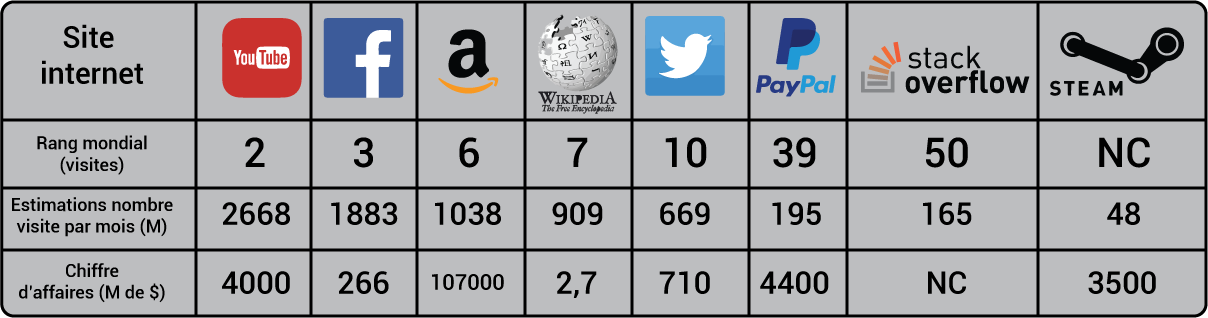
\includegraphics[width=17cm]{figures/topWebsites}
  \caption{Quelques chiffres sur les géants du net}
  \label{fig:top-sites}
\end{figure}

Nous avons analysé les plus vastes sites internet mondiaux. Tout le monde les connaît ou en a déjà entendu parlé, à part peut-être Stackoverflow, qui est un forum d’entraide concentré sur la programmation dans tous les langages, et Steam, qui est une plate-forme de vente de jeux vidéos dématérialisés. Ces sites ont des points communs et des particularités que nous avons décortiqués afin d’en extraire des idées, tout en essayant à chaque fois de mesurer leur pertinence par rapport à notre application. Il en a résulté la figure suivante.


\begin{figure}[h]
  \centering
  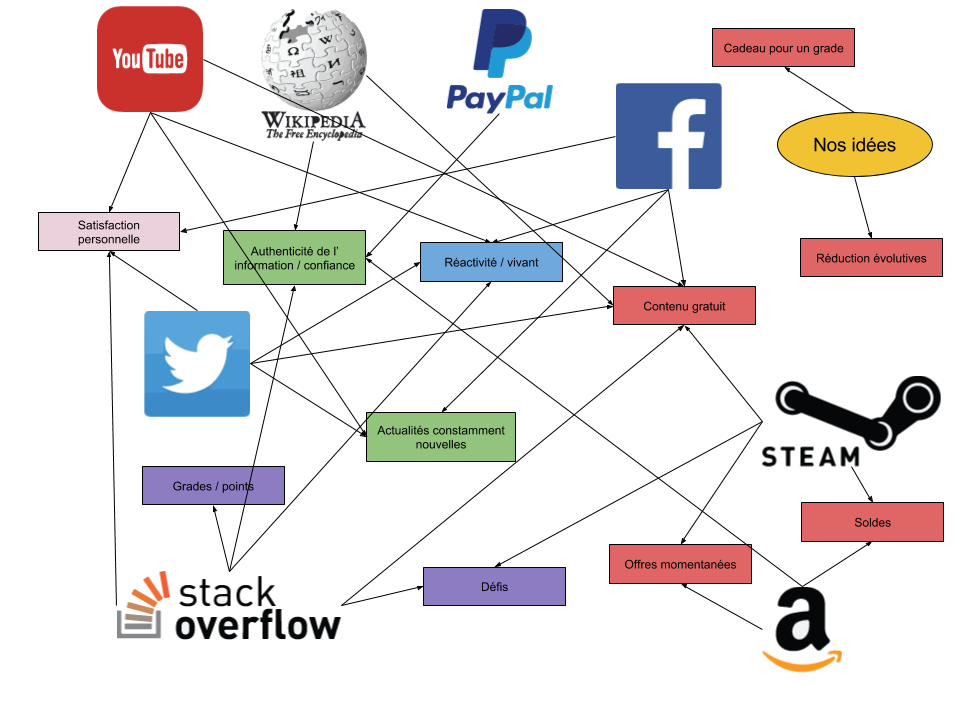
\includegraphics[width=17cm]{figures/site_idea}
  \caption{Idées tirées des sites}
  \label{fig:site-idea}
\end{figure}

\subsection{Résultats de la recherche}

Un concept important est la gratuité de l’application, au moins au début de l’utilisation ou pour son lancement. Si l’utilisateur doit payer pour y accéder, il aura moins tendance à l’essayer. Fournir un certain contenu gratuit dés son inscription est également un moyen de le motiver, et forcer un achat risque de faire fuir l’utilisateur. Il faut toujours attirer les utilisateurs et réussir à les fidéliser petit à petit pour leur montrer qu’ils ont besoin de l’application qu’ils utilisent.

Dans la continuité de ce principe, on peut également offrir des cadeaux aux utilisateurs, ou des réductions qui arrivent petit à petit en fonction de leur fréquence d’utilisation de l’application. Ils seront ainsi plus motivés à continuer et obtenir ces réductions, même si au départ cela ne leur était pas indispensable.

Une autre idée importante qu’on a pu dégager de ces sites internet est l’accomplissement de soi et la satisfaction personnelle que cela peut nous apporter. Internet met en contact des milliers de personnes et l’on peut aider les autres assez rapidement si on en a l’envie. Sans obligations, de nombreuses personnes vont aider les autres car cela leur fait juste plaisir.

Les défis peuvent pousser les utilisateurs à se surpasser, et effectuer des tâches sans s’en rendre compte. On trouve ce principe dans les succès sur Steam, ces actions à effectuer dans un jeu qui n’apporte rien d’autre que la fierté d’avoir réussi à les réaliser. Cette idée est liée avec l’idée de grades et de points, permettant de mettre en confrontation les utilisateurs et les pousser à devancer les autres. Nous allons grâce à ces deux idées compléter les attentes des personnes correspondant aux archétypes des leaders et des explorateurs.

\newpage
\section{Fonctionnalités de l’application}


Il nous a fallu organiser nos tâches par niveau de priorité afin de ne pas se perdre dans le code, c’est pourquoi nous avons fait cette carte heuristique, d’abord, sur un tableau à l’école, puis nous avons numérisé toutes ces idées.
\begin{figure}[h]
  \centering
  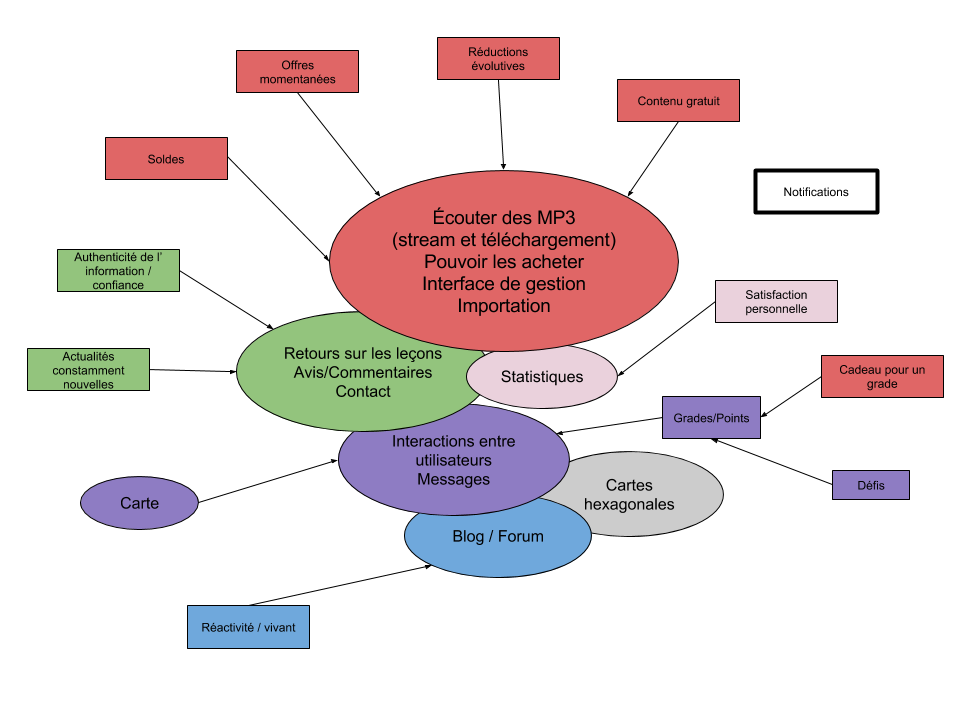
\includegraphics[width=17cm]{figures/vue_ensemble}
  \caption{Carte heuristique de l'application}
  \label{fig:ensemble-view}
\end{figure}


\subsection{Écouter des mp3, achat et importation}

La fonctionnalité primaire de l’application était bien évidemment d’écouter les mp3 des leçons de notre encadrant sur l’application. Cependant, les lecteurs de musiques réalisés avec Ionic n’étaient pas très exploitables (style non adapté, ou ne fonctionnaient pas) il a donc fallu en réalisé un “home made”. Comme les mp3 ne sont pas gratuits pour la plupart, il s’agissait aussi de pouvoir les acheter, nous avons donc réfléchi aux possibilités de paiement via une application et deux solutions étaient envisageables : Paypal, ou un paiement intégré à l’application passant par le Playstore (ou l’AppStore pour les utilisateurs d’iPhone).
(import ???)

\subsection{Retours sur les leçons, commentaires, contact}

Ensuite, il était évident que l’application ait un coté social, pour que l’utilisateur puisse se sentir écouté, que la communauté soit active, et que certains des points de motivation soient bien présents. C’est pourquoi il est possible de laisser des commentaires sur leçons ainsi qu’une note entre 0 et 5. Aussi, sur le site déjà existant il était possible d’envoyer un mail à M. Latocha via la partie contact, et nous avons pensé qu’il était important que cette partie demeure présente sur l’application.  (confirmer quand sera fait ???)

\subsection{Interactions entre les utilisateurs}

Outre les commentaires, une idée primordiale selon nous pour rendre une application motivante était les échanges entre utilisateurs, avec la possibilité d’envoyer des messages privés ; les profils ne seraient alors pas anonymes et chaque utilisateur posséderait un compte personnel et une page profil (comme sur la plupart  des réseaux sociaux actuels).

\subsection{Statistiques et objectifs}

Une autre idée qui nous est venue à l’esprit était d’afficher des statistiques, car ils sont un moteur de la motivation ; en effet, un utilisateur qui voit qu’il a effectué un cours et observe une évolution de son graphique personnel, ainsi que l’augmentation d’un score qui lui serait attribué en fonction des heures qu’il passe à faire des cours, peut lui donner envie de pratiquer encore plus, ou de revenir chaque jour sur l’application.

\subsection{Blog ou Forum}

On arrive maintenant dans les fonctionnalités un peu plus facultatives, mais auxquelles on a pensé car une partie identique était déjà présente sur le site existant mais aussi car c’est le principe de base du site Stackoverflow. Le principe serait de remplir cette partie avec des topics contenant une question suivi d’une succession de réponses pouvant être écrites par tous les utilisateurs. Enfin, nous avons pensé à intégrer une carte sur l’application car la localisation est une option présente sur beaucoup de réseaux sociaux, et, dans notre cas, elle apporterait l’avantage de savoir qui pratique aussi le Feldenkrais autour de chez soi : les utilisateurs pourraient alors organiser des rencontres entre eux pour pratiquer ou débriefer sur des leçons.


\subsection{Autres fonctionnalités}

Dans les fonctionnalités également facultatives nous avons pensé à des cartes hexagonales pour présenter les cours, dans le style d’un jeu vidéo (les cours seraient une sorte de quête à accomplir pour avancer comme sur un plateau de jeu) et les couleurs des cours pourraient s’actualiser quand celui-ci est acheté, et ensuite accompli. Néanmoins c’est une tâche demandant beaucoup de boulot et cette fonctionnalité serait peu adaptée aux petits écrans.

\chapter{Organisation}

\section{Méthode de travail}

Nous avons dans un premier temps défini les leviers de motivation que l’on voulait inclure dans l’application. Nous avons ratissé toutes les possibilités que l’on a pu imaginé durant cette période pour pouvoir avoir une vue globale de toute ce qui était utilisé. Nous avons ainsi pu choisir au mieux les principes à adopter. Nous avons ensuite sélectionner ceux qui nous paraissaient les plus pertinents. A partir de cette liste de critères, nous avons imaginé les fonctionnalités qui pouvait s’y appliquer. L'intérêt de cette méthode et de pouvoir savoir pour une fonctionnalité sera présente dans l’application plutôt qu’une autre, et ainsi savoir au mieux l’impact que celle-ci va avoir sur l’utilisateur. Ainsi, une liste de toutes les fonctionnalités principales a été crée. Celles-ci ont été ensuite regrouper dans différents groupes, en fonction du thème de celle-ci, et de son importance dans le projet. Nous voulions partir d’un noyau de base constitué des fonctionnalités les plus importantes. A ce noyau ce sont rattaché les autres fonctionnalités de moins en moins prioritaires. Ceci nous a donc permis de développer les fonctionnalités dans leur ordre d’importance et ainsi arriver petit à petit au prototype qui était prévu.

\section{Technologies utilisées}

\begin{wrapfigure}{r}{6cm}
  \centering
  
\includegraphics[width=5cm]{figures/ionic}
  \caption{Logo de Ionic}
  \label{fig:logo-ionic}
\end{wrapfigure}
Le résultat qui était à fournir à l’issu de ce projet était un prototype d’application. Nous avons donc choisi des technologies permettant de réaliser rapidement un prototype qui fonctionne. Pour la partie application, nous avons utilisé Ionic. Cette technologie permet de programmer une application en utilisant les technologies du web, c’est à dire HTML, CSS et Angular.JS principalement. Elle est également gratuite et dispose une belle interface utilisateur. Elle est Open Source et son ergonomie ressemble grandement à une application native. De plus, sa communauté active permet la résolution rapide des problèmes rencontrés. Elle dispose de fonctionnalités natives qui y sont intégrées et est également compatible avec la technologie Cordova qui nous as permis de disposer de toutes les fonctionnalités natives d’Android, comme par exemple l’écoute de fichiers audios, qui est la fonctionnalité principale de l’application.

\newpage
\begin{wrapfigure}{l}{6cm}
  \centering
  
\includegraphics[width=6cm]{figures/node}
  \caption{Logo de Node.JS}
  \label{fig:logo-nodejs}
\end{wrapfigure}
Pour ce qui concerne le serveur, nous avons utilisé le langage Node.JS. Celui-ci permet d’avoir une API REST, c’est-à-dire un certain nombre d’URL correspondant chacune à une tache spécifique à effectuer, comme par exemple la création d’un élément ou la récupération de tous les éléments de la base de données. Ainsi, chaque fois que l’on envoie une requête au serveur, celui-ci va récupérer les données nécessaires, effectuer des traitements sur celles-ci et modifier la base de données s’il le faut, puis renvoyer le résultat au client, c’est-à-dire l’application mobile. Un avantage de ce principe de serveur et qu’il pourra tout aussi bien être utilisé dans une application mobile qu’un site web.
\\
\\
\begin{wrapfigure}{r}{6cm}
  \centering
  
\includegraphics[width=6cm]{figures/materialize}
  \caption{Logo de Materialize}
  \label{fig:logo-materialize}
\end{wrapfigure}

Grâce à ce serveur, nous avons pu développé, en plus de l’application mobile, une interface d’administration permettant à notre encadrant de créer et uploader les leçons sur le serveur et qui sont directement accessibles via l’application. Pour réaliser le design de cette partie d’administration, nous avons utilisé le framework materializecss. Celui-ci nous a permi de rendre l’interface épuré et clair, permettant ainsi de gérer au mieux les cours disponibles pour les utilisateurs.
\\
\\
\\
\begin{wrapfigure}{l}{6cm}
  \centering
  
\includegraphics[width=6cm]{figures/mariadb}
  \caption{Logo de MariaDB}
  \label{fig:logo-mariadb}
\end{wrapfigure}

Pour stocker les données de l’application, nous avons utilisé le système de gestion de base de données MariaDB. Celui-ci est Open Source et gratuit, et est utilisé par un grand pourcentage des sites internets car il est très répandu et sa communauté est grande et active. Afin de faire la liaison entre Node.JS et MariaDB, nous avons utilisé l’ORM Sequelize qui permet d’utiliser le principe d’Active Record qui lie ainsi tables de la base de données et objets en mémoire. Ainsi, une table de la base corresponds exactement à un objet sur lequel des fonctions de recherche ou de sauvegarde ont été rajoutées. Nous pouvons ainsi modifier ces objets et les sauvegarder directement dans la base de manière aisée et efficace. De plus, si nous avons une association entre plusieurs tables, l’objet correspondant possède également les méthodes pour récupérer les autres objets associès.




Les données utiles transitent entre ces deux parties sous le format JSON qui est un format de plus en plus courant de nos jours depuis l’apparition de Node.JS. En effet, ce format permet de communiquer facilement entre le client et le serveur car ils sont tous les deux basés sur du javascript, et ce dernier arrive très bien à comprendre le JSON et utiliser le contenus des données en tant que variables. Cette étape de communication est donc très rapide et ne nous encombre pas avec des fonctionnalités de parsing à rajouter.


\section{Répartition des tâches}

La répartition des tâches changeaient de temps en temps pour nous permettre d’avoir une vue globale de l’application. Nous ne voulions pas qu’une seule personne soit au courant d’une seule partie de l’application sans avoir d’idée sur le reste de celle-ci. Nous voulions donc être informés à tout moment de ce qui était fait, et nous avons beaucoup travaillé de paire. Un bon exemple est la réalisation d’une quelconque fonctionnalité. La plupart du temps, nous réfléchissions ensemble sur les informations nécessaires à cette fonctionnalité, puis à une interface qui lui correspondrait. Ensuite les deux parties, application et serveur, étaient codées en parallèle. Enfin, nous faisions la liaison entre les deux et nous corrigions respectivement les erreurs.


\section{Technique}

Nous avons séparé tout notre code dans 3 gits différents. Ainsi, nous avions un dépôt qui concernait l’application mobile, et un autre concernant le serveur. Nous testions tout d’abord l’application grâce à une sorte d’émulateur offert par ionic qui permet d’ouvrir notre application dans un navigateur web. Cependant, certaines fonctionnalités natives comme la lecture de musique était indisponible durant le test sur navigateur. Il nous fallait forcément tester l’application sur nos téléphones portables. Le fait d’avoir séparer le serveur de l’application mobile nous a permis de déployer le serveur sur un serveur de test afin de l’utiliser avec l’application mobile. De ce fait, notre téléphone pouvait se connecter à ce serveur web car il n’était pas hébergé sur nos ordinateurs, inaccessibles de l’extérieur. Le dernier dépôt quant à lui nous a servi pour l’élaboration du rapport. Il est plus logique de le séparer du reste du code car il ne le concerne pas directement.

\begin{wrapfigure}{r}{6cm}
  \centering
  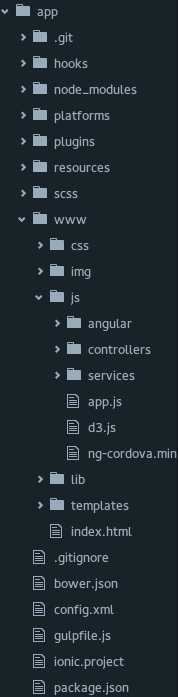
\includegraphics[width=5cm]{figures/tree_app}
  \caption{Arborescence de l'application}
  \label{fig:tree-app}
\end{wrapfigure}

\newpage
Le dossier principal concernant le développement est le dossier www, car il contient tous les fichiers nous permettant de donner vie à l’application. Les autres dossiers sont principalement là pour faire marche de manière général ionic et les différents plugins qui ont pu être ajoutés. Le dossier templates nous permet de définir toutes les vues de l’application, la forme de celle-ci. Ainsi, toutes les pages visibles par l’utilisateur sont dans ce dossier. Le dossier js nous permet quant à lui de définir les différentes actions associés à ces vues, c’est-à-dire tous les contrôles disponibles, le fond de l’application. Les deux parties sont liés dans les templates. Nous pouvons définir pour chaque boutons quelle est la fonction qui sera exécuté lors du clic sur celui-ci. Ainsi, lorsque qu’un utilisateur réalise une action, une fonction contenu dans fichier du dossier controllers va se mettre en marche. Si celle-ci a besoin de joindre le serveur afin de récupérer des données ou d’en ajouter dans la base de données, elle fera appel à une autre fonction contenu dans le dossier services. Ainsi, l’application est découpée selon le patron de conception Modèle (services) - Vue (templates) - Contôleur (controllers).

Les dossiers img et css contiennnent les différentes images visibles sur le site, ainsi que les éléments de design spécifiés en CSS. Le fichier index.html contenu à la racine du dossier www permet d’inclure tous les fichiers que nous avons réalisé dans tous les autres dossier et ainsi lier l’application ensemble. Celui-ci définit également les menus permettant d’accéder au vue.
\newpage


\begin{wrapfigure}{r}{6cm}
  \centering
  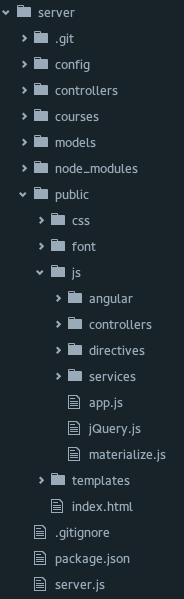
\includegraphics[width=5cm]{figures/tree_server}
  \caption{Arborescence du serveur}
  \label{fig:tree-server}
\end{wrapfigure}
Le dossier templates corresponds au dossier www qui se situe dans l’arborescence de l’application. Il est constitué des mêmes fichiers et du même fonctionnement et ne sera pas donc plus explicité ici.

Le dossier config contient les différents fichiers de configuration. C’est-à-dire un fichier comportant les différents paramètres d’accès pour la connexion à la base de données. Il contient un fichier “router” définissant toutes les routes accessibles dans l’API. Chaque route est liée à une fonction d’un contrôleur qui va effectuer le traitement des données envoyées. Chacune des routes possède un paramètre indiquant si oui ou non l’utilisateur doit être authentifié pour y accéder, nous permettant de couper correctement l'accès au personnes non autorisées. Ces routes nous permettent donc de bien structurer notre application pour la rendre la plus propre possible.

Du fait que le serveur soit une API REST le serveur ne prend que les parties Modèle (models) et Contrôleur (controllers) du patron de conception MVC. Le dossier models définit les différents objets que nous auront besoin de stocker. Dés que nous lançons le serveur pour la première fois, Sequelize va parcourir ces fichiers pour créer les tables de la base de données correspondantes à chacun des objets. C’est fonctionnalité nous est très utile lors du développement car nous n’avons pas à se soucier de la synchronisation de nos deux bases de données, et également lors du déploiement sur un serveur.

Les contrôleurs quant à eux vont recevoir la requête du client, qui est passée par les routes, et aura la possibilité de récupérer les paramètres de celle-ci. Une vérification de ces paramètres va être effectuée afin d’être sûr qu’ils sont corrects. Par la suite, il va traiter ces paramètres, soit en faisant une recherche, soit en insérant des données dans la base. Par la suite, il va renvoyer une réponse qui corresponds à ce que le client attends, comme par exemple une liste d’objets qui seront affichés.

\chapter{Solution proposée}
Quand l'utilisateur lance l'application, il va arriver sur l'interface ci-contre. Il pourra alors choisir de s'inscrire s'il n'a pas déjà un compte, ou de se connecter à un compte existant.

\begin{figure}[h]
  \centering
  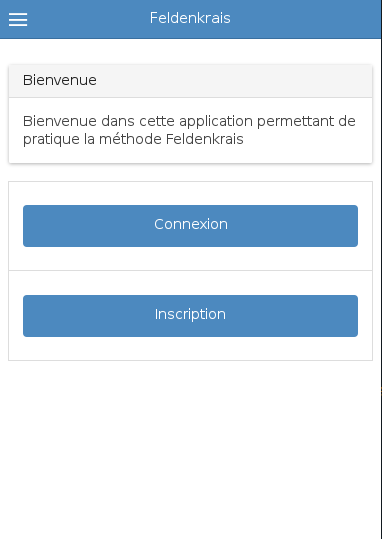
\includegraphics[width=4cm]{figures/accueil}
  \caption{Accueil}
  \label{fig:accueil}
\end{figure}
Si il choisi de s'inscrire, il pourra alors entrer un login, son adresse email pour pouvoir être contacté par la suite s'il poste des commentaires, et son mot de passe ainsi que la confirmation de celui-ci afin de s'assurer qu'il ne s'est pas trompé en l'écrivant. En s'inscrivant, le serveur va créer son compte et le connecter directement après.

\begin{figure}[h]
  \centering
  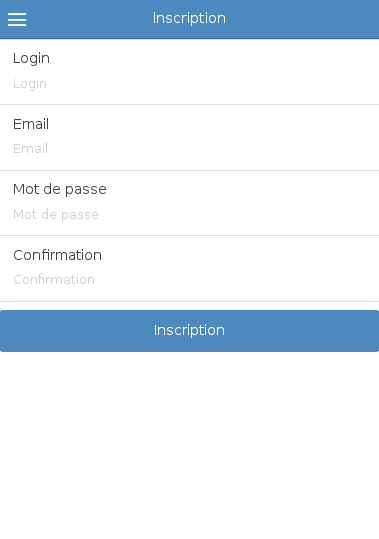
\includegraphics[width=4cm]{figures/inscription}
  \caption{Inscription}
  \label{fig:inscription}
\end{figure}
\newpage
Si l'utilisateur choisit de se connecter, il pourra entrer son login ainsi que son mot de passe. Une fois connecté, il n'auras plus besoin de se connecter à chaque fois qu'il lance l'application et pourra également y accéder sans avoir accés à Internet.

\begin{figure}[h]
  \centering
  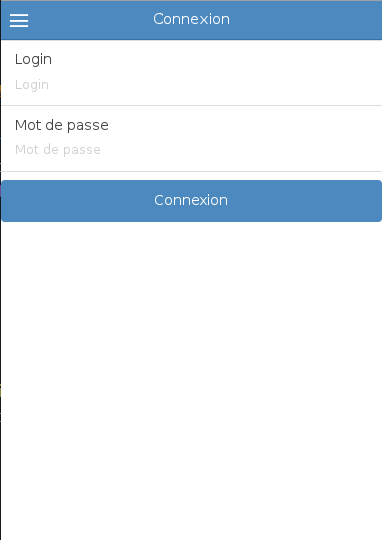
\includegraphics[width=4cm]{figures/connexion}
  \caption{Connexion}
  \label{fig:connexion}
\end{figure}
Une fois connecté, l'utilisateur arrive sur la liste des actualités. Celles-ci sont créées par l'administrateur, c'est à dire notre encadrant.

\begin{figure}[h]
  \centering
  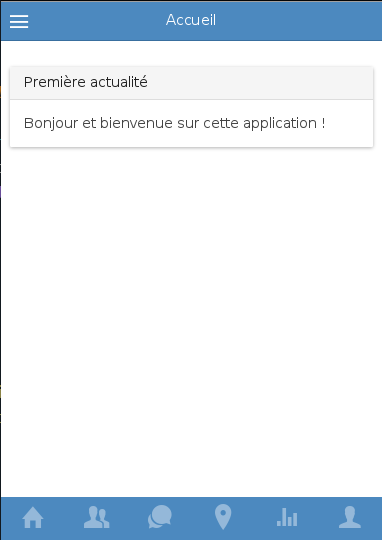
\includegraphics[width=4cm]{figures/news}
  \caption{Actualités}
  \label{fig:news}
\end{figure}
\newpage
Il pourra ensuite aller sur la liste des packs de leçons, lui permettant de choisir un pack gratuit qu'il débloque par défaut, ou de parcourir les différents packs payants qui sont disponibles et les acheter s'ils le désirent.

\begin{figure}[h]
  \centering
  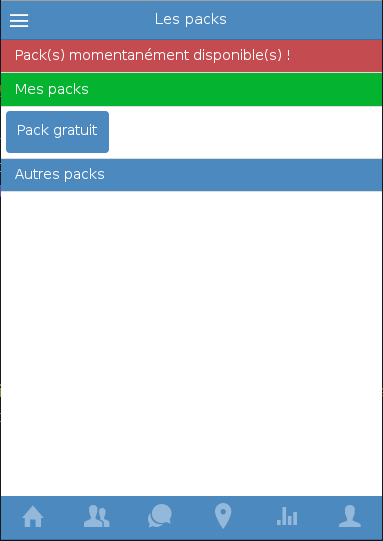
\includegraphics[width=4cm]{figures/packs}
  \caption{Liste des packs de leçons}
  \label{fig:packs}
\end{figure}
Il peut également aller sur la page de stats afin de renseigner son objectif à accomplir, c'est à dire un nombre de leçon à faire par jour, par semaine ou par mois, selon son choix.

\begin{figure}[h]
  \centering
  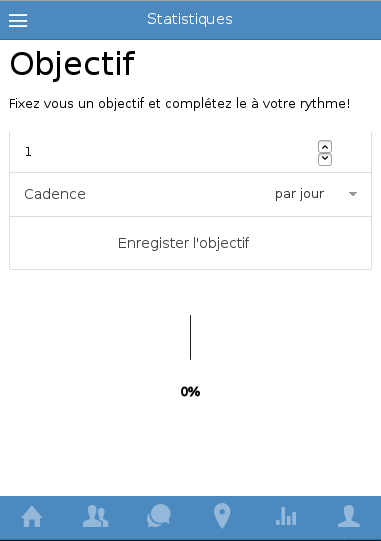
\includegraphics[width=4cm]{figures/stats}
  \caption{Objectif}
  \label{fig:stats}
\end{figure}
\newpage

\section{Résultats actuels}

Nous disposons actuellement d’un prototype d’application permettant d’écouter des leçons en streaming. Elle permet aussi d’avoir des statistiques par rapport à l’objectif que l’on s’est fixé, afin de se motiver et d’effectuer des leçons régulièrement.

La partie d’administration est composée de la création des différents packs de cours et les cours avec pour information le prix du pack, ainsi que sa disponibilité, le nom du pack, le nom de chaque cours, et leur durée et le fichier audio associé. Il est également possible d’ajouter des actualités qui apparaîtront à tous les utilisateurs lors de leur connexion.

Ce projet nous a permis personnellement de mieux utiliser la technologie Ionic et également se spécialiser dans Angular.JS. Nous avons également découvert des outils permettant de gérer au mieux la conception et la réalisation d’un projet, et ainsi de savoir s’organiser et ne pas se perdre dans l’étendu de celui-ci, et dans les contraintes techniques associées.

\section{Perspectives}

Les principales perspectives de l’application consiste à développer les différntes fonctionnalités qui ont été imaginées mais qui ne sont pas encore présentes dans celle-ci. Nous pourrions également mettre le prototype à l'essai pour quelques pratiquants afin qu'ils le testent quelques temps pour obtenir des retours et ainsi savoir quelles améliorations nous pourrions faire.




\listoffigures



\end{document}
